\documentclass[11pt,twoside=true]{scrartcl}
\usepackage[utf8]{inputenc}
\usepackage[english, ngerman]{babel}
\usepackage{amsmath,amsthm,verbatim,amssymb,amsfonts,amscd, graphicx}
\usepackage{graphicx}
\usepackage{siunitx}
\usepackage{mhchem}
% \usepackage[T1]{fontenc}
% \usepackage{charter}
\usepackage[bitstream-charter]{mathdesign}
\usepackage[hyperref=true,
            url=false,
            isbn=false,
            backref=true,
            % style=science,
            citereset=section,
            maxcitenames=3,
            maxbibnames=100,
            block=none,
            backend=biber]{biblatex}

\addbibresource{sources.bib}

%% floatrow
\usepackage{floatrow}
\floatsetup{valign=c, heightadjust=all}
\newfloatcommand{capbtabbox}{table}[][\FBwidth]
%%

%% MATH COMMANDS
\newcommand{\dd}[2]{\frac{d{#1}}{d{#2}}}
\newcommand{\e}{\mathrm{e}}

\usepackage[%
  bookmarks, % Create bookmarks
  bookmarksopen=true, % Unfold bookmatk tree in PDF viewer when document is opened
  bookmarksopenlevel=1, % Level of unfolding
  bookmarksnumbered=true, % Number bookmarks
  hidelinks, % do not highlight hyperlinks -- looks ugly
  pdfpagelabels=true, % See manual...
  plainpages=false, % See manual...
  hyperfootnotes=true, % Hyperlinks for footnotes
  hyperindex=true, % Indexeinträage verweisen auf Text
]{hyperref}
\usepackage{wrapfig}


\setkomafont{section}{ \LARGE\bf }
\setkomafont{title}{ \Large\bf }
\setkomafont{section}{ \Large\bf }
\setkomafont{subsection}{ \normalfont\bf }



\titlehead{
    
\includegraphics[width=5cm]{./figures/luh_logo.pdf}
  
}

\title{Praktikumsbericht}
\subtitle{Erzeugung ultrakurzer Laserpulse (IQ 7)}
\author{Jonathan Rossberg,
      Eduard Sauter}
\date{\today}
\dedication{Praktikum im Rahmen der Vorlesung Koheränte Optik im
Sommersemester 2016 \\
Betreuer: Bernhard Kreipe}


\begin{document}

\maketitle
\newpage
\section{Dauerstrichbetrieb}
\textsl{Bestimmen sie den theoretischen Verlauf der $g_0-P$ Kennlinie} 
%
Die Ratengleichungen lauten.
\begin{align*}
  T_R \dd{g}{t} & 
    = \underbrace{\frac{g_0}{T_L}}_{\text{Pumpen}}   
    - \underbrace{\frac{g P}{ P_{\text{sat}}}}_{\text{Stimulierte Emission}}  
    - \underbrace{\frac{g}{T_L}}_{\text{Dunkle Abregung}} \\
  T_R \dd{P}{t} & 
    = \underbrace{2 g P}_{\text{Stimulierte Emission}}  
    + \underbrace{2 g P_\text{vac}}_{\text{Spontane Emission}}  
    - \underbrace{\frac{P}{T_p}}_{\text{Lineare Verluste}}
\end{align*}


Im Dauerstrichbetrieb sind $\dd{g}{t} = \dd{P}{t} = 0$. 
Man erhält dann
%
\begin{align*}
  2 g_s P_s  & = \frac{P_s}{T_p} - 2 g_S P_\text{vac} \\
  - \frac{g_0}{T_L}  & = g_s\left( \frac{P_s}{P_\text{sat}} - \frac{1}{T_L} \right) \\
  & \iff  \\
  g_s & = \frac{1}{2 T_p} \frac{1}{1- \frac{P_\text{vac}}{P_S}} = \frac{g_0}{1 - \frac{P_S T_L}{P_\text{sat}}} \\
  & \iff   \\
  \left( 1 - \frac{P_S T_L}{P_\text{sat}} \right)  & = g_0 2 T_p \left( 1 - \frac{P_\text{vac}}{P_S} \right) \\
  & \iff  \\
  0 & = P_s^2 + P_s (2 g_0 T_p - 1) \frac{P_\text{sat}}{T_L} - \frac{P_\text{vac}P_\text{sat}}{T_L}
  & \iff \\
  P_S & = - \frac{\gamma}{2} \pm \sqrt{\frac{\gamma^2}{4} + \delta}
\end{align*}
Mit 
%
\begin{align*}
  \gamma = \frac{P_\text{sat}}{T_L} (2 g_0 T_p - 1) && \delta = \frac{P_\text{vac} P_\text{sat}}{T_L}
\end{align*}
%
Die Form dieser Kennlinien sind in Abbildung \ref{fig:lasing_pvac} dargestellt.
%
Für $P_\text{vac} = 0 $, also vernachlässigung von spontaner Emission ergibt sich
%
\begin{align*}
  P_s = \frac{P_\text{sat}}{T_L} (2 g_0 T_p - 1) && g_s = \frac{1}{2 T_p}
\end{align*}
%


Die Lasingbedingung ist in diesem Fall eine positive stationäre Leistung
$P_s > 0$ und führt zu
%
\begin{align*}
  g_0 T_p > \frac{1}{2}
\end{align*}
%
\begin{figure}
  \centering
  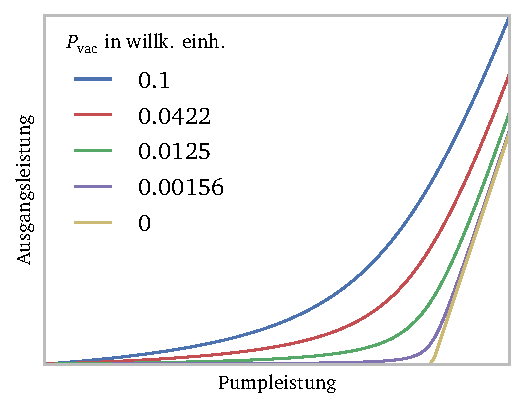
\includegraphics[width=0.5\textwidth]{./figures/lasing_pvac.pdf}
  \caption{Laserkennlinie für verschiedene koeffizienten der spontanten
  Emission}
  \label{fig:lasing_pvac}
\end{figure}

Bei gegebenem Gesamtverbrauch $g_s=l$ ist dann außerdem die Lebenszeit der Photonen
pro Resonatorumlauf $T_p = \frac{1}{2 l}$. 

Man aus den Ratengleichungen qualitativ sehen, dass bei einer Störung von $P'<P$
der Gewinn größer wird und dadurch auch $P'' > P'$. Das System ist also stabil unter
Störung von $P$ durch z.B. einen akusto-optischen Modulator (siehe kommenden Abschnitt).

\newpage


\subsection{Schwellenstrom und Slope-Efficiency}
Zuerst wird der Laser mit einem hochreflektierenden Spiegel ($R > 0.99$) betrieben.
Die Ausgangsleistung des Lasers wurde in abhängigkeit des Pumpstroms mit einem 
Thermischen Leistungsmesskopf ermittelt. Danach wurde der Strahl des Pumplasers
ausgekoppelt und dasselbe für den Pumplaser wiederholt, um dann durch den Fit
aus dem ersten Graphen den differentiellen Wirkungsgrad zu erhalten. Beide
Messungen sind in Abbildung \ref{fig:slope_efficiency} veranschaulicht.

\begin{figure}
  \centering
  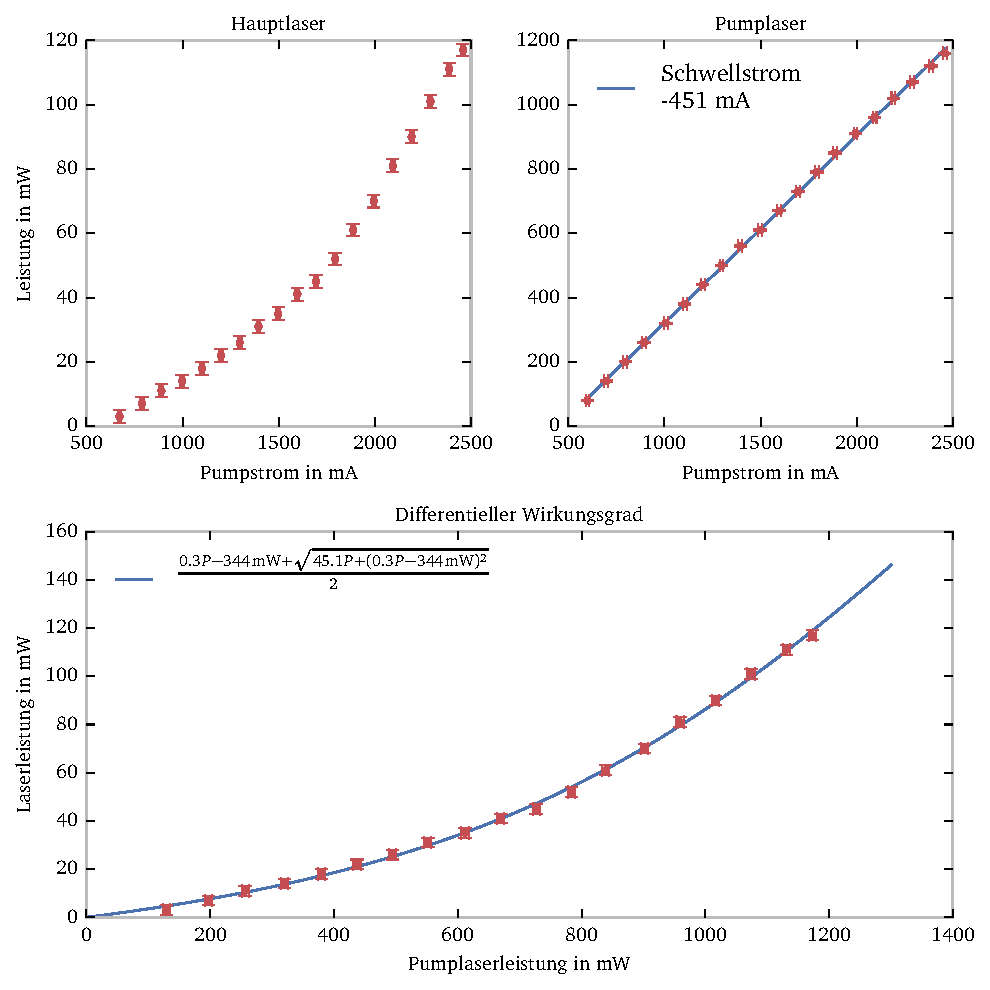
\includegraphics[width=1\textwidth]{./figures/slope_efficiency.pdf}
  \caption{Differentieller Wirkungsgrad. An der ersten Kurve erkennt man
  dass der Laser erst bei der Schwelle des Pumplasers Leistung gewinnt. Im
  unteren Graphen ist dieser Effekt nicht mehr zu sehen da die echte
  Pumpleistung als Argument aufgetragen worden ist. An dem unteren Graphen
  sieht man, dass die Lösung der Ratengleichung für einen kleinen Wert von
  $P_\text{vac}$ einen guten Fit für die Laserleistung liefert. Dies ist auch
  durch den hochreflektierenden Auskoppelspiegel begründet, durch den die
  spontante Emission entscheidender wird.  Für kleine Intensitäten ist der
  verwendete thermische Messkopf nicht sensitiv genug gewesen.}

  \label{fig:slope_efficiency}
\end{figure}

\subsection{Auskopplungsstärke}
Der hochreflektierende Auskoppler ist in diesem Versuch durch andere Auskoppelspiegel
mit definierten Transmissionswerten ausgetauscht worden. Aus den $P-I$  Diagrammen
wurden die Schwelleistungen durch lineare extrapolation bei Größeren Pumpleistungen
ermittelt. Diese Schwelleistungen sind in Findlay-Clay darstellung in Abbildung
\ref{fig:findlay_clay} zu sehen. Die Verluste pro Rundgang sind das Verhältnis
der Fitkoeffizienten und sie ergeben sich zu \SI{65}{\percent}. 
\begin{figure}[h!]
  \centering
  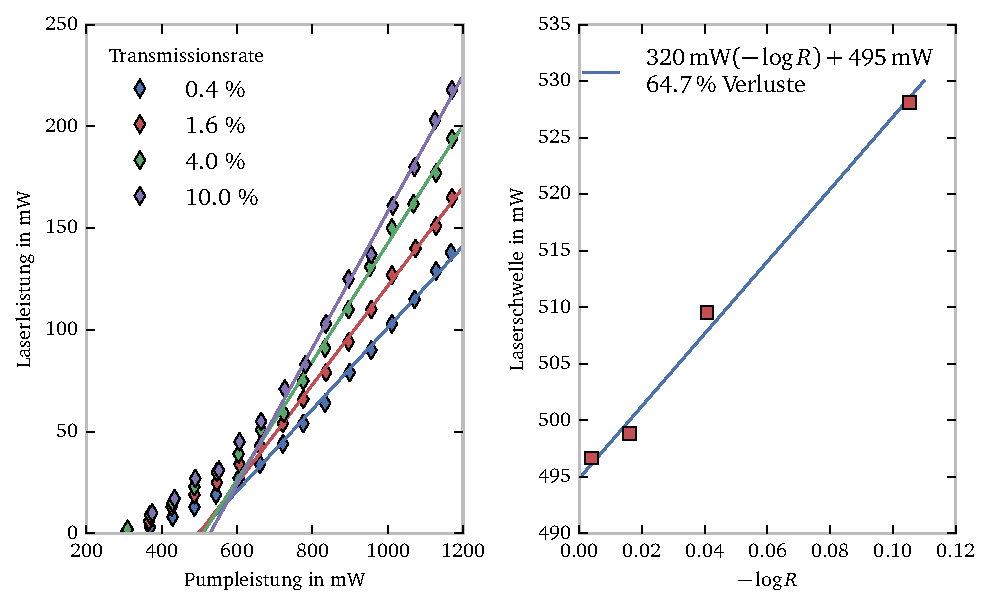
\includegraphics[width=1\textwidth]{./figures/findlay_clay.pdf}
  \caption{Findlay-Clay darstellung der Laserschwellen}
  \label{fig:findlay_clay}
\end{figure}

\subsection{Störung des stabilen Betriebs}
Mithilfe eines Opto-Akustischen Modulators kann der stabile Laserbetrieb gestört
werden. Der AOM ändert seinen Brechungsindex je nach angelegter Spannung. In unserem 
Fall wurde mit einem Frequenzgenerator eine Rechtecksfunktion erzeugt, die man
in Abbildung \ref{fig:relaxation_osci} sehen kann.
\begin{figure}[h!]
  \begin{floatrow}
    \ffigbox{
      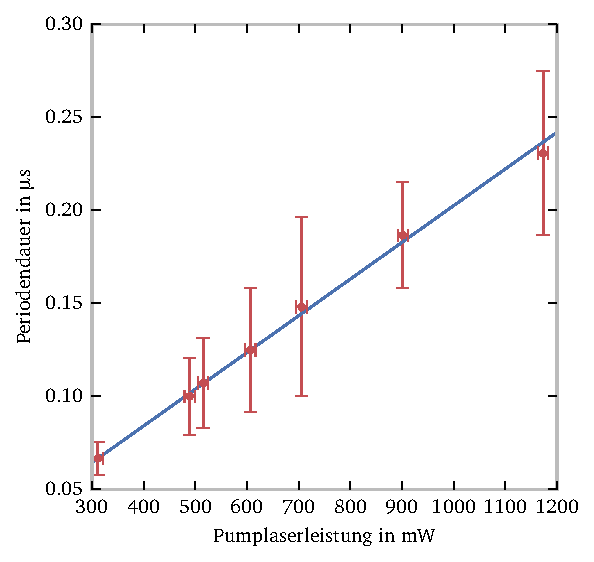
\includegraphics[width=\linewidth]{./figures/relaxationsschwingung.pdf}
    } {
      \caption{Frequenz der Relaxationsschwingungen als Funktion der Pumpleistung. Die Unsicherheiten
      ergaben sich je nachdem wieviele Perioden auf dem Display abgelesen werden konnten}
    }
    \ffigbox{
      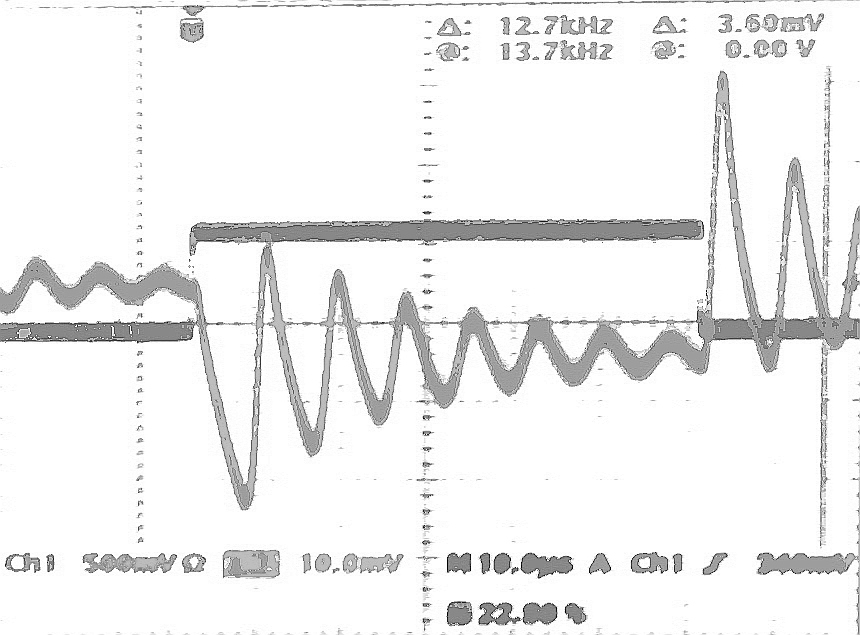
\includegraphics[width=\linewidth]{./figures/relaxation_osci.jpg}
      \label{fig:relaxation_osci}
    } {
      \caption{Anzeige des Oszilloskops mit den beobachteten Relaxationsschwingungen bei
      der an den AOM angelegten Rechtecksfunktion.}
    }
  \end{floatrow}
\end{figure}


\subsection{Transversale Moden}
Bei nicht optimaler justierung waren auch andere Moden zu erkennen als die 
Grundmode $\text{TEM}_{00}$. Sie wurden mit einer Handykamera abfotografiert und
für Abbildung \ref{fig:tem10} und \ref{fig:tem20} nachbearbeitet. Es wurden 
Hermite-Moden beobachtet, was für eine rechteckige Symmetrie des Lasers spricht. 

\begin{figure}[h!]
  \begin{floatrow}
    \ffigbox{
      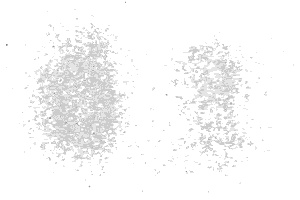
\includegraphics[width=\linewidth]{./figures/tem10.JPG}
    } {
      \caption{TEM$_{10}$ Mode}
      \label{fig:tem10}
    }
    \ffigbox{
      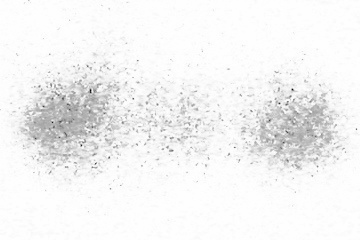
\includegraphics[width=\linewidth]{./figures/tem20.JPG}
    } {
      \caption{TEM$_{30}$ Mode}
      \label{fig:tem20}
    }
  \end{floatrow}
\end{figure}

\section{Erzeugung der 2. Harmonischen}
\subsection{Intensität und Fokushärte}
Die Intensität des Frequenzverdoppelten Strahls wurde mithilfe eines
Photomultipliers vermessen. Der vorhandene thermische Messkopf zur Leistungsmessung
war nicht sensitiv genug um damit die Leistung direkt zu vermessen zu können.


\begin{figure}[h!]
  \begin{floatrow}
    \ffigbox{
      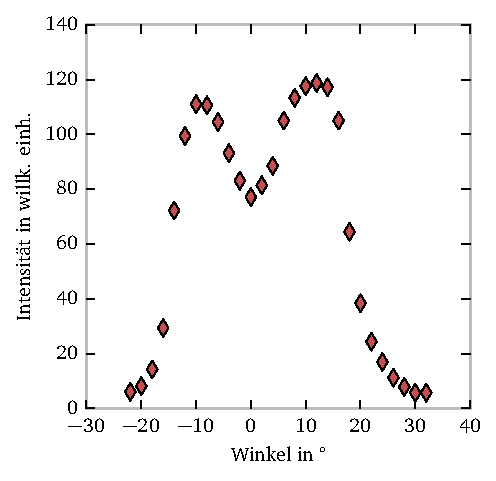
\includegraphics[width=\linewidth]{./figures/angle_shg.pdf}
    }
    {%
      \caption{Transversalwinkelabhängigkeit SH-Intentensität. Die Funktion
      ist symmetrisch erwartet worden. Vermutlich hat die Verschiebung vom Fokus
      weg beim Rotieren des Kristalls diese Symmetrie gebrochen. }
      \label{fig:angle_shg}
    }
    \capbtabbox{%
      \begin{tabular}{c c c c c c}
        \hline\hline
        Brennweite $f$ in \SI{}{\milli\metre} & Intensität in w. E. \\
        \hline
        30 & 150 \\
        40 & 145.2 \\
        80 & 134.2 \\
        100 & 117 \\
        \hline\hline
      \end{tabular}
    }{%
      \caption{Stärke der zweiten Harmonischen unter verschiedenen Brennweiten
    bei Fokussierung in den BBO Kristall.}
    }
  \end{floatrow}
  \end{figure}
  

\subsection{Strahlradius im Fokus mit Rasierklingenmethode}
Die Intensität des Gaußschen strahls kann durch
%
\begin{align*}
  I(r, z) = I_0\left( \frac{w_0}{w(z)} \right)^2 \e^{\frac{-2 r^2}{w^2(z)}}
\end{align*}
%
beschrieben werden. Dabei ist der Strahlradius der Punkt an
dem die Transversale funktion auf $1/\e^2$ abgefallen ist. Sie ist 
nach \cite{gaussbeamwiki} gegeben durch
%
\begin{align*}
  w(z) = w_0 \sqrt{1 + \left( \frac{z}{z_R} \right)^2} && z_R = \frac{\pi w_0^2}{\lambda}
\end{align*}
%
für große $|z|$ ist der Verlauf in guter Näherung linear,
%
\begin{align*}
  w(z) \approx w_0 \frac{z}{z_R} = \frac{\lambda z}{w_0 \pi} = \sin{\theta} 
                      \overset{\theta \ll 1}{\approx} \theta
\end{align*}
%
man kann also durch die Steigung experimentell den Strahldurchmesser
am Fokuspunkt ermitteln. Für kleine Werte ist diese gleich dem Divergenzwinkel
$\theta$. 

Um den Strahldurchmesser zu bestimmen wird eine Rasierklinge horizontal und
vertikal durch den Strahl gefahren. Der Intensitätsverlauf hinter der Klinge
entspricht einem Integral über eine Gaußfunktion. Diese Funktion wurde auch
als Fit für die Abbildungen \ref{fig:beam_div} verwendet.
%
\begin{align*}
  \operatorname{erf}(x) = \int_{-\infty}^{x} e^{-\gamma^2} d\gamma
\end{align*}
%


\begin{figure}[h!]
  \centering
  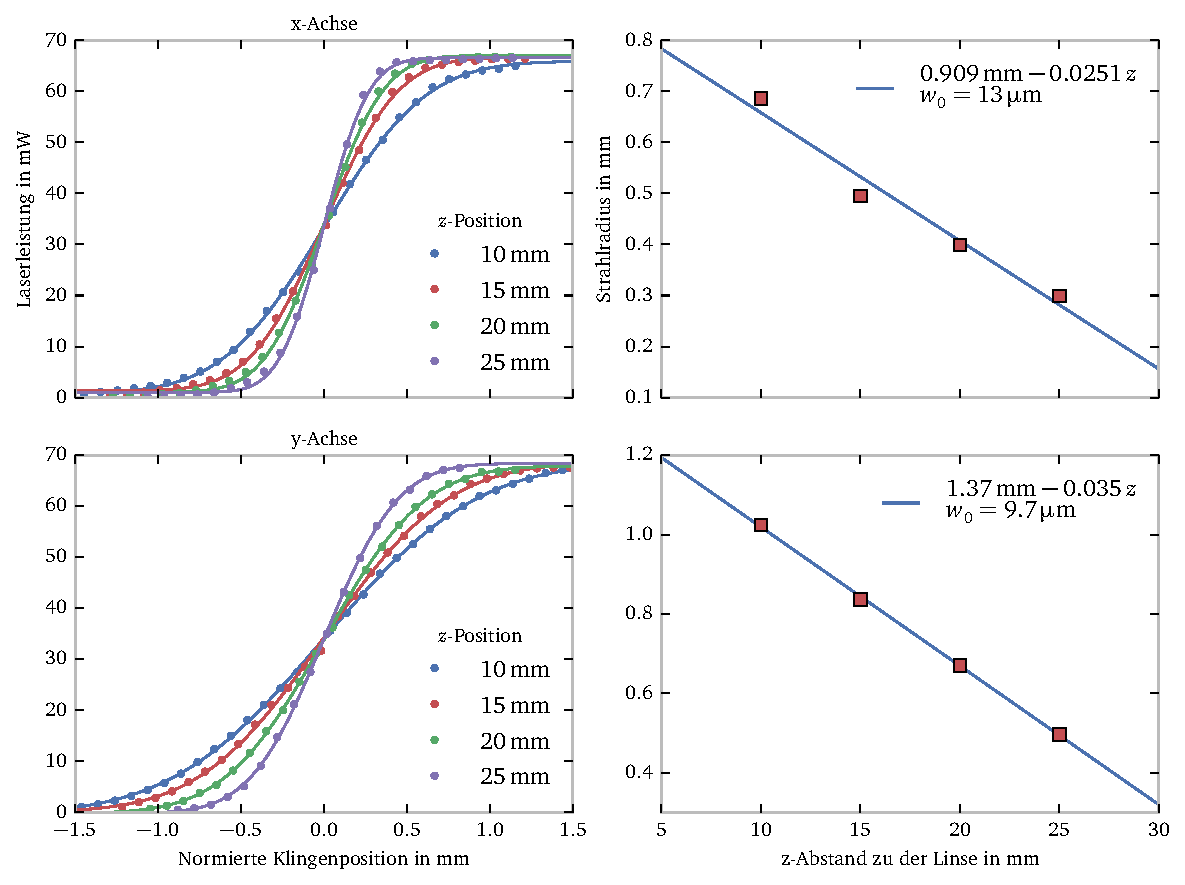
\includegraphics[width=1\textwidth]{./figures/beam_div.pdf}
  \caption{Strahldurchmesser und Intensitätsprofile. Der Strahl wurde mit einer
  \SI{40}{\milli\metre} Linse fokussiert. Vor dem Fokus wurden für verschiedene 
  Abstände zur Linse die ersichtlichen Graphen gemessen. Der Strahl}
  \label{fig:beam_div}
\end{figure}






\end{document}
